\section{Case Study 1: Publication Data}

TimeSets can be applied to domains requiring the understanding of temporal events including history, movies, publications, etc. Figure~\ref{fig:teaser} shows a timeline of the CIA leak case~\cite{CIA2007} covering both time-point and interval events happening from 2002 to 2007. In this section, we choose another domain, academic publications, to demonstrate TimeSets. A subset of 200 publications with the most citations is extracted from the IEEE InfoVis articles~\cite{Stasko2013}. Each publication is assigned one or many \textit{concepts} such as \textit{network} or \textit{evaluation}. We use concept as the set attribute to group publications. Figure~\ref{fig:citations} shows the visualization of this dataset. No aggregation is needed when producing the layout, only complete and trimmed labels are displayed in the visualization.

\begin{figure*}[ht]
\centering
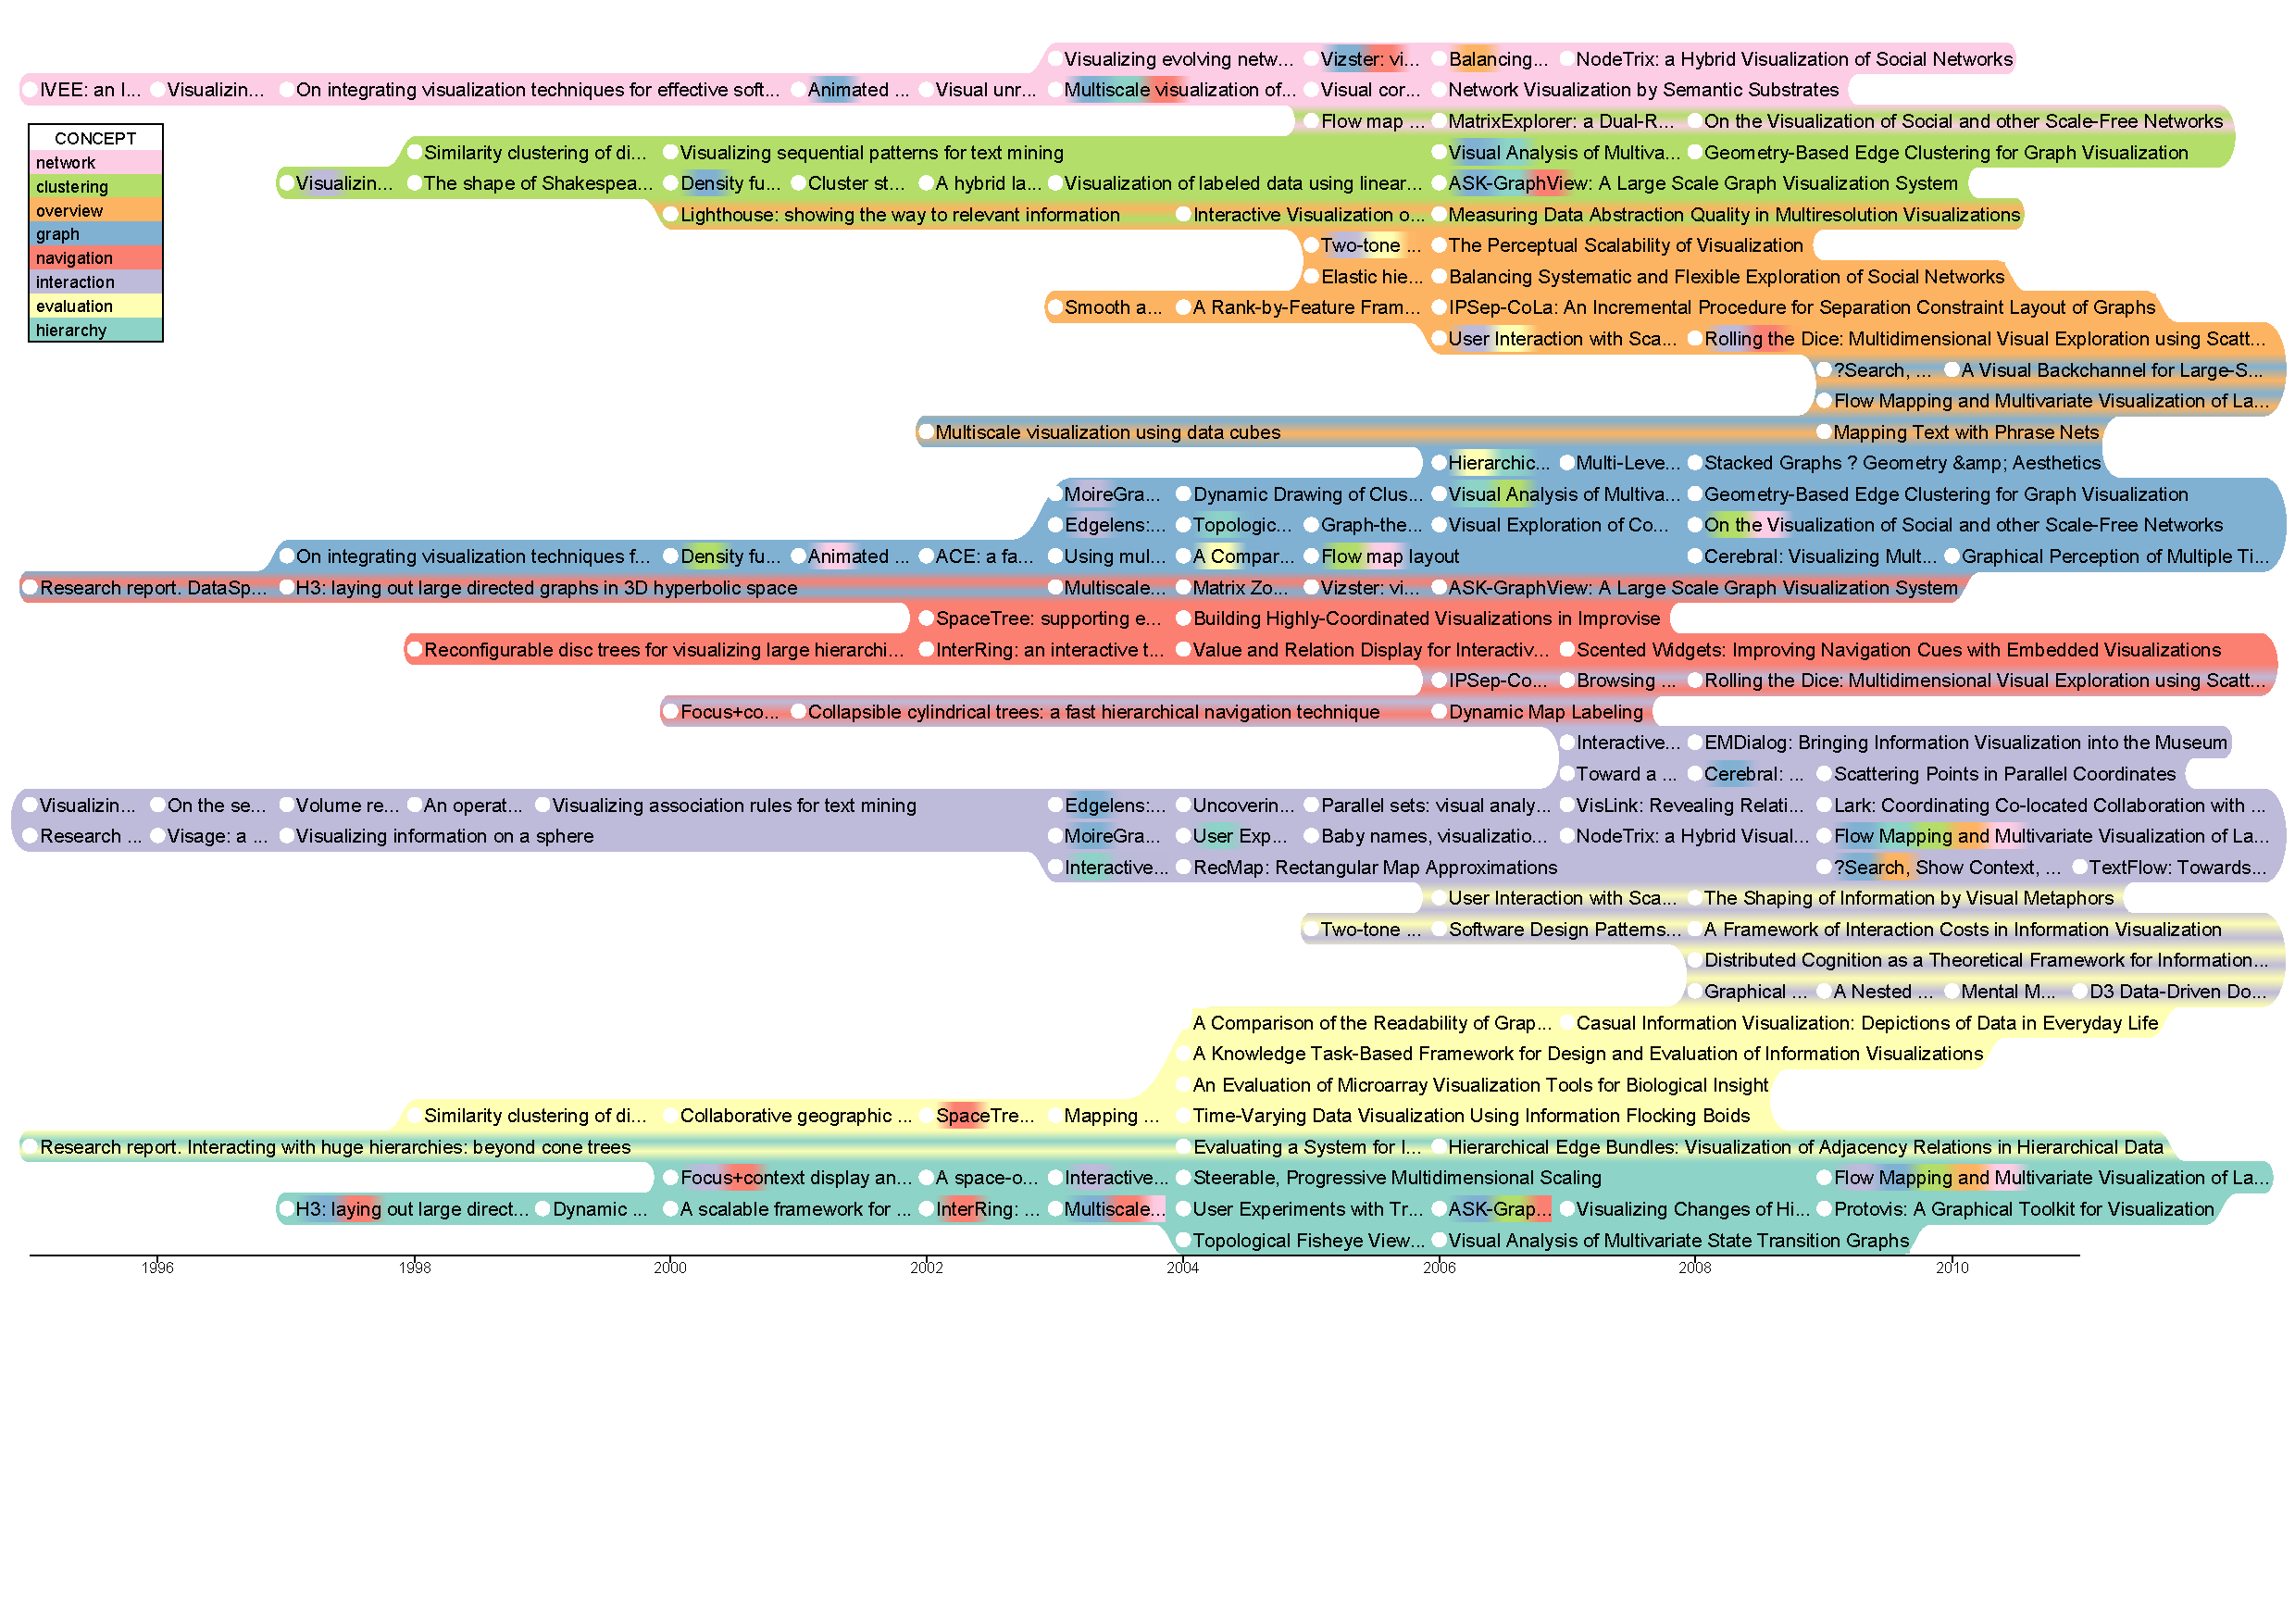
\includegraphics[width=\linewidth]{figure13}
\caption{TimeSets visualization of 200 publications with the most citations in the IEEE InfoVis conference from 1995 to 2013. Concepts are used to group publications and only eight concepts appearing most in those publications are shown (see the legend in the top left corner).}
\label{fig:citations}
\end{figure*}

TimeSets can show distribution of categorical data over time as in ThemeRiver~\cite{Havre2002}. A quick glance at the visualization brings us a surprise. There is much void space on the left as opposed to a very dense area on the right indicating that there are many more highly cited papers published in the last ten years of the dataset than in the first ten years. This trend also holds for individual concepts. Each colored band starts with a single row and increases its height towards the end of the timeline. This observation is in contrast with the common thought: papers published in a longer time would have more citations. One possible explanation is that the IEEE InfoVis conference accepts more papers over time -- in the dataset, there are 18 articles in 1995 while 37 articles in 2013. Another reason could be that publications in the last ten years are really of high quality.

TimeSets cannot show all intersections among sets; however,  its layout maximizes the number of shared elements between two neighboring sets. As a result, the visible intersections usually have the most elements among all intersection. In the visualization, the most notable gradient area is the intersection between yellow and purple sets implying that there are many excellent papers focusing on both \textit{evaluation} and \textit{interaction}. Another observation at the top of the visualization with three concepts: \textit{network}, \textit{clustering} and \textit{overview} with clustering is in between the other two. This is expected because clustering techniques are important in visualizing large networks or getting the overview of a large dataset.

In this figure, TimeSets uses the color gradient method to show full memberships of multi-set elements. For instance, inside the pink band (\textit{network} papers), there are quite a few small blue gradients (\textit{graph} papers). This is sensible because the closeness between these two concepts and they may often appear together in a paper. Another interesting observation is at the bottom band -- \textit{hierarchy}. The last paper ``Flow Mapping and Multivariate Visualization...'' includes five concepts: \textit{hierarchy} (blue background) and \textit{interaction}, \textit{graph}, \textit{overview} and \textit{network} (small gradients).